\chapter{Derivace}

\vfill{}
{\Huge\color{gray} \begin{equation*}
    \diff{}{x} \left( \sin \alpha^2 \right) = 2 \alpha \cos \alpha^2
\end{equation*} }

\vfill{}
\pagebreak
\section{Definice}

\subsection{O~čem se budeme bavit?}

\textit{Derivace}, někdy též \textit{diferenciál}, vyjadřuje, v~jaké míře jistá
funkce $f$ roste či klesá. Derivace je takový prostředek, který umožňuje, pokud
možno, pro všechna $x \in \mathcal{D}(f)$ určit, jakým způsobem funkce roste či
klesá.

Určit, jak funkce roste či klesá, je dost obtížné. Máme ale přímku. Je-li přímka
grafem jisté funkce $g(x) = ax + b$, za~míru růstu resp.~poklesu funkčních hodnot
můžeme označit koeficient~$a$, tj. směrnici přímky, která je grafem funkce $g$.
Grafem funkce je ale většinou křivka.

To ničemu nevadí -- ke~křivce jsme schopni zkonstruovat tečnu prakticky kdekoliv se
nám zachce -- a~tečna je již přímka. Můžeme tedy prohlásit, že křivka v~určitém bodě
roste stejnou mírou, jako tečna v~tom stejném bodě.

\begin{figure}[hb!]
    \centering
    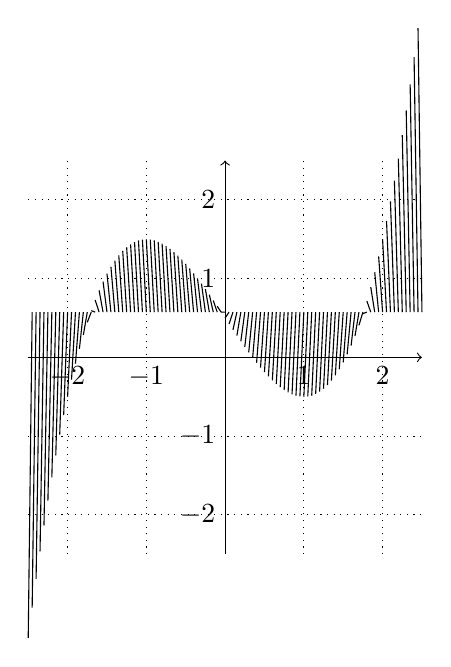
\begin{tikzpicture}
    % Svislá mřížka
    \foreach \x in {-2,...,2} {
        \ifnum \x = 0 {} \else {
            \draw[dotted] (\x, -2.5) -- (\x, 2.5);
            \draw (\x, 0) node[anchor=north] {$\x$};
        } \fi
    }
    % Vodorovná mřížka
    \foreach \y in {-2,...,2} {
        \ifnum \y = 0 {} \else {
            \draw[dotted] (-2.5, \y) -- (2.5, \y);
            \draw (0, \y) node[anchor=east] {$\y$};
        } \fi
    }
    % Osa x a y
    \draw[->] (-2.5, 0) -- (2.5, 0);
    \draw[->] (0, -2.5) -- (0, 2.5);

    % Graf s 100 vzorků
    \foreach \xa in {-2.5, -2.45,...,2.5} {
        \def \xb {\xa + 0.05}
        \def \ya {\xa^3 / 2 - \xa * 3 / 2 + 1 / 2}
        \def \yb {\xb^3 / 2 - \xb * 3 / 2 + 1 / 2}
        \draw (\xa,\ya) -- (\xb,\yb);
    }
\end{tikzpicture}
    \caption[
        Ukázka, jak by derivace měla fungovat
    ]{
        Ukázka, jak by derivace měla fungovat. Všimněte si, jak sklon tečny, který
        je definovaný jako směrnice ekvivalentní lineární funkce je funkční hodnotou
        funkce $f'(x)$.
    }
\end{figure}

Všimněte si, že hodnotám $x \in \mathcal{D}(f)$ určíme maximálně jedno reálné číslo,
které určuje strmost grafu funkce $f$. Výstupem derivace je proto nějaká jiná funkce,
kterou označíme jako $f'$, jejíž funkční hodnota reprezentuje právě strmost grafu
původní funkce $f$.

Z~výše uvedených vlastností, které by derivace měla mít, vyplývá několik dalších
důležitých vlastností:
\begin{enumerate}
    \item Derivaci jsme schopni určit pouze u~spojitých funkcí, přesněji pouze
    u~spojitých úseků, ve kterém mohou být díry ve formě izolovaných bodů, kde
    funkce není definována.
    \item Směrnice tečny určuje, jestli graf funkce roste či klesá:
    \begin{itemize}
        \item Je-li směrnice kladná, graf zde určitě roste.
        \item Analogicky je-li směrnice záporná, graf zde určitě klesá.
        \item Je-li tečna kolmá k~ose $x$, tj. rovnoběžná s~osou $y$, nejsme
        schopni tečnu zapsat pomocí lineární funkce, jejíž grafem je tečna
        sama, nejsme schopni určit míru růstu a derivace zde bude nedefinovaná.
        \item Je-li tečna v~určitém bodě grafu vodorovná s~osou $x$, směrnice
        musí být nulová. Pozor -- to však ještě neznamená, že je v~blízkosti
        tohoto bodu funkce kostantní (nalezení takových funkcí nechávám jako
        úlohu).
    \end{itemize}
    \item Nechť $\mathcal{F}$ je množina všech funkcí $f: \reals \to \reals$.
    Poté se na~derivaci můžeme dívat jako na~zobrazení množiny $\mathcal{F}$
    do~množiny $\mathcal{F}$.
    \item $\mathcal{D}(f') \subset \mathcal{D}(f)$. To vyplývá z~faktu, že funkci
    $f'$ přiřazujeme hodnotu pro určité $x$, pokud vůbec, pouze pokud je $f(x)$
    definované.
\end{enumerate}

\begin{exercise}
    Nalezněte alespoň jednu funkci, jejíž derivace v~určité hodnotě $x$ je nulová,
    tj. směrnice tečny grafu v~daném bodě je nulová a přesto nemůžeme v~sebemenším
    okolí prohlásit funkci jako konstantní. Takových funkcí je nekonečně mnoho.
    Nápověda: Začněte od těch nejjednodušších funkčních předpisů -- i~tam najdete
    takové případy.
\end{exercise}

\subsection{Formální zápis}

Nakonec bychom si řekli, jak vztah, že funkce $f'$ je derivací (diferenciálem) funkce
$f$, zapsat. Vztah mezi funkcemi $f$ a~$f'$ budeme zapisovat tímto způsobem:
\begin{equation*}
    \diff{f}{x} = f'
\end{equation*}
Proč tento velmi zvláštní zápis? To rozebereme v~následujícím oddílu. Zastavme se
však na chvíli.

Prozatím jsme se omezovali jen na~funkci, kterou jsme označili většinou jako $f$,
a~řekli, že její derivace bude označená stejně, ale bude tam mít navíc čárku,
např.~$f'$. Pokud však budeme derivovat spíše výraz, než-li funkci, bude lepší, když
použijeme nějaký vhodný přímý zápis, než abychom pokaždé museli říct, že výraz je
funkčním předpisem nějaké funkce. Proto by se nám hodil způsob, jak zapsat derivaci
výrazu (který funkce stejně představuje). Existuje hned několik zavedených způsobů.
\begin{align*}
    \diff{}{x} \left( \frac12 x - 3 \right)                 & = \frac12 &
    \frac{\text{d} \left( \frac12 x - 3 \right)}{\text{d}x} & = \frac12 &
    \left( \frac12 x - 3 \right)'                           & = \frac12
\end{align*}
Všechny tři formy zápisu vyjadřují, že diferenciál výrazu $\frac12 x - 3$
v~závislosti na~$x$ je konstanta rovna $\frac12$. Nejčastěji se využívá možnost vlevo
-- umožňuje přehlednější zápis i mnohem složitějších výrazů. Možnost vpravo se
nevyužívá, je-li ve vzorci více proměnných (resp.\ argumentů funkce), na~jejichž
závislosti jsme schopni derivovat.

\subsection{Derivace jako podíl dvou malých změn}

Mějme příklad, ve~kterém budeme chtít vědět okamžité zrychlení auta v~daném časovém
momentě. Začněme však průměrným zrychlením. Fyzika v~případě změny (skoku) hodnoty
jisté proměnné používá velké řecké písmeno delta, např. $\Delta v$ by mohlo
představovat změnu rychlosti a~$\Delta t$ změnu času, tj. délku jistého časového
úseku. Proto pro~průměrné zrychlení auta určitého měřeného časového úseku, označme
jej $a_{\text{avg}}$,  bychom napsali:

\begin{equation*}
    a_{\text{avg}} = \frac{\Delta v}{\Delta t}
\end{equation*}

Konkrétně, pokud by auto zrychlilo o~7,2~km/h~=~2~m/s za půl vteřiny, platilo by, že
$\Delta v~= {2 \text{ m}/\text{s}}$ a~$\Delta t = {0,5 \text{ s}}$. Proto by průměrné
zrychlení během takové doby bylo
\begin{equation*}
    a_{\text{avg}}
    = \frac{\Delta v}{\Delta t}
    = \frac{2 \text{ m} \cdot \text{s}^{-1}}{0,5 \text{ s}}
    = 4 \text{ m} \cdot \text{s}^{-2}\text{.}
\end{equation*}

Zároveň, pokud auto zpomalí, rozdíl rychlostí je záporný, takže i~zrychlení je
záporné. Nicméně se však jedná o~průměrné zrychlení. Pokud cheme okamžité zrychlení,
musíme učinit pár úprav. Musíme změřit rychlost v~měřeném časovém úseku pokud možno
co nejvícekrát, aby průměrné zrychlení v~době mezi dvěma sousedními měřeními
rychlosti se co nejvíce blížilo okamžitému zrychlení.

To nám umožňuje zavést okamžité zrychlení jako funkci závislou na~čase, zrovna tak
i~okamžitou rychlost. Snažili bychom se funkční předpisy pro okamžitou rychlost
$v(t)$ a~okamžité zrychlení~$a(t)$ vyjádřit co nejpřesnějším funkčním předpisem
na~základě naměřených dat. Funkce $v(t)$ a~$a(t)$ budou tedy spojité a~pomocí tečen
jsme schopni určit graf derivace obou funkcí.

Ale zároveň si povšimněme, že pokud budou naše měření přesnější a~přesnější, poté se
každá přímka vedoucí skrz jakékoliv dva sousední body bude stále více a~více
přibližovat tečně ke~grafu funkce -- a~toho využijeme.

Označme si nepatrnou změnu
rychlosti jako $\text{d} v$ místo $\Delta v$. Ta bude kladná při zrychlování
a~záporná při zpomalování. Velmi malý časový úsek mezi měřeními jako $\text{d} t$
místo $\Delta t$. Tehdy bude okamžité zrychlení v~daném čase $t$ rovno
\begin{equation*}
    a(t) = \diff{v}{t}(t)
\end{equation*}
a~tento poměr velmi malých hodnot bude velmi dobře odhadovat směrnici tečny a~tudíž
i~hodnotu derivace funkce $v(t)$. Z~toho vyplývá, že derivací funkce $v(t)$ je tedy
funkce $a(t)$. Nyní již stačí tuto myšlenku formalizovat. Předtím ale ještě pár úloh.

\begin{exercise}
    Mějme funkci $s(t)$ určující, jakou vzdálenost jsme ujeli za určitý čas. Jaká
    funkce (veličina) je derivací funkce $s(t)$?
\end{exercise}

\begin{exercise}
    Pohybová (kinetická) energie je závislá na~rychlosti pohybu daného tělesa, rovněž
    jako hybnost. Hmotnost tělesa se standardně nemění. Jaký vztah je mezi kinetickou
    energií a~hybností? V~případě, že si již vzorce nepamatujete či je neznáte,
    můžete využít internetu. Nápověda: Nakreslete si graf hybnosti a~kinetické
    energie v~závislosti na~rychlosti pro předem danou hmotnost do~jedné soustavy
    souřadnic.
\end{exercise}

\subsection{Formální definice}

Opět máme funkci $f$, jejíž derivací je funkce $f'$. Abychom formálně definovali
derivaci musíme nejlépe sestrojit výraz, který je roven $f'$. K~tomu potřebujeme dvě
hodnoty na~ose $x$, z~nichž spočítáme funkční hodnoty a~$f'$ bude rovno podílu
rozdílu funkčních hodnot a rozdílu argumentů (těch dvou hodnot na~ose $x$). Přitom
ale potřebujeme vyjádřit, čím blíže jsou ty dvě hodnoty na~ose $x$, tím více se
k~derivaci blížíme. K~tomu využijeme limitu:

\paragraph*{Definice:} Funkce $f'$ je derivací funkce $f$, pokud platí, že:
\begin{equation*}
    f'(x) = \lim_{a \to x} \frac{f(x) - f(a)}{x - a}
\end{equation*}

Tato definice je sice správná, ale není v~ní příliš vidět ten náš malý rozdíl mezi
dvěma hodnotami na~ose $x$ -- v~našem případě proměnných $x$ a~$a$. Proto určíme
rozdíl $h = a - x$ a~přepíšeme zlomek tak, abychom nepoužili proměnnou~$a$.
Po~určitých úpravách dostaneme odlišný výraz:

\paragraph*{Definice:} Funkce $f'$ je derivací funkce $f$, pokud platí, že:
\begin{equation*}
    f'(x) = \lim_{h \to 0} \frac{f(x + h) - f(x)}{h}
\end{equation*}

S~tímto zápisem se zřejmě setkáte častěji.

\vfill{}
\pagebreak
\section{Diferenciál lineární funkce}

Derivace lineární funkce je jednoduchá. Grafem lineární funkce je přímka, u~níž růst
umíme vyjádřit směrnicí, což u~vyjádření pomocí funkčního předpisu odpovídá
koeficientu přítomnému u~lineárního členu. Proto pro lineární polynomy platí:
\begin{equation*}
    \forall a, b \in \mathbb{R}: \diff{}{x} \left( ax + b \right) = a
\end{equation*}

\begin{exercise}
    Vypočítejte diferenciál následujících lineárních funkcí:
    \begin{align*}
        f(x) &= 2x + 3
        & k(x) &= \frac{3}{2} \left( x + \frac{\pi^2}{7} \right) 
        & n(x) &= 5x \sqrt{2} + 3 \sqrt[3]{3} \\
        g(x) &= -4x + \frac{5}{6}
        & \ell(x) &= \frac{5}{7}x + \frac{1}{\pi}
        & p(x) &= k(x) + \ell(x) \\
        h(x) &= -\frac{4}{\pi}x + \frac{\sqrt{2}}{3}
        & m(x) &= \pi x + 2
        & q(x) &= f(x) + g(x) + n(x)
    \end{align*}
\end{exercise}

\section{Diferenciál mocninné funkce}

Pokračujme mocninnými funkcemi (tj. funkcemi ve~tvaru $f(x) = ax^m$). Takovou funkci
zderivujeme tak, že ji nejprve vynásobíme exponentem mocniny a~následně exponent
snížíme o~jedničku. Tento postup platí pro exponent v~oboru všech reálných čísel.
Tomuto pravidlu říkáme \emph{řetězové pravidlo}. Formálněji jsme schopni výrokem
zapsat toto pravidlo:
\begin{equation*}
    \forall a, m \in \mathbb{R} :
    \diff{}{x} \left(ax^m\right) = amx^{m - 1}
\end{equation*}

Zkusme nějaký příklad. Mějme funkci $f(x) = 3x^5$. Tu chceme zderivovat. Nejprve tedy
celý výraz vynásobíme exponentem. Dostaneme tedy výraz $15x^5$. Nyní stačí
od~exponentu odečíst jedničku. Poté tedy vznikne funkce $f'(x) = 15x^4$, která je
derivací funkce $f(x)$, tedy můžeme zapsat:
\begin{equation*}
    \diff{}{x} \left( 3x^5 \right) = 15x^4.
\end{equation*}

\begin{exercise}
    Spočítejte diferenciál (derivaci) výrazů uvedených níže. Nezapomeňte, že každou
    konstantu $k$ lze vyjádřit jako $kx^0$, kde $x$ jste schopni zaměnit
    za~jakoukoliv jinou proměnnou. Taktéž každou odmocninu jsme schopni zapsat jako
    mocninu.
    \begin{align*}
        &\diff{}{t} \left( \frac38 t^8 \right) &
        &\diff{}{x} \left( \sqrt{x} \right) &
        &\diff{}{z} \left( 2,7z \right) &
        &\diff{}{v} \left( \frac12 mv^2 \right) \\
        &\diff{}{x} \left( \pi \right) &
        &\diff{}{h} \left( 120h \right) &
        &\diff{}{s} \left( 8s^2 \right) &
        &\diff{}{q} \left( 8q \right)
    \end{align*}
\end{exercise}

\subsection{Mocninné funkce geometricky}

Nyní se pokusme řetězové pravidlo zobrazit geometricky. Nejdříve si to ukážeme pro
druhou mocninu.

Nechť máme čtverec se~stranou o~proměnné délce $x$. Obsah tohoto čtverce jsme schopni
spočítat pomocí vzorce. Nechť tedy funkce $S(x) = x^2$ počítá obsah čtverce. Co se
stane, když jisté $x$ zvětšíme o~nepatrnou změnu $\text{d}x$? Poté se nám změní
i~povrch čtverce. Označme změnu plochy čtverce jako $\text{d}S$. Nyní si problém
zobrazíme geometricky. Stranu čtverce jsme zvětšili o~$\text{d}x$ a~nový čtverec
vhodně oddělili na~čtyři části:

\begin{figure}[H]
    \centering
    \begin{tikzpicture}
    \filldraw[fill=lightgray, draw=black] (0, 0) rectangle (4, -4);
    \draw (2, -2) node[anchor=center] {\huge $S(x)$};
    \filldraw[fill=orange, draw=black] (4.1, 0) rectangle (4.5, -4);
    \filldraw[fill=orange, draw=black] (0, -4.1) rectangle (4, -4.5);
    \filldraw[fill=purple, draw=black] (4.1, -4.1) rectangle (4.5, -4.5);
    \draw [decorate, decoration = {calligraphic brace, amplitude=.3cm}] (4.6, 0) --  (4.6,-4);
    \draw (4.9, -2) node[anchor=west] {$x$};
    \draw [decorate, decoration = {calligraphic brace, amplitude=.1cm}] (4.6, -4.1) --  (4.6,-4.5);
    \draw (4.7, -4.3) node[anchor=west] {$\text{d}x$};
    \draw [decorate, decoration = {calligraphic brace, amplitude=.3cm}] (4, -4.6) -- (0, -4.6);
    \draw (2, -4.9) node[anchor=north] {$x$};
    \draw [decorate, decoration = {calligraphic brace, amplitude=.1cm}] (4.5, -4.6) -- (4.1, -4.6);
    \draw (4.3, -4.7) node[anchor=north] {$\text{d}x$};
\end{tikzpicture}
    \caption{
        Geometrická představa čtverce, jehož stranu~$x$ jsme zvětšili
        o~$\text{d}x$. Na~obrázku je záměrně $\text{d}x$ příliš veliké -- to kvůli
        názornosti.
    }
\end{figure}

Původní čtverec je zobrazen šedě a~nové přírůstky jsou zobrazeny barevně. Takto jsme
schopni schopni vyjádřit změnu obsahu $\text{d}S$ pomocí barevně vyznačených oblastí
v~obrázku a~vyjádřit derivaci vydělením $\text{d}x$:
\begin{equation*}
    \text{d}S = 2 \cdot {\color{orange} x \, \text{d}x} + {\color{purple} \text{d}x^2} \quad \implies \quad
    \diff{S}{x} = 2x + \text{d}x
\end{equation*}
Ale máme menší problém -- přebývá nám tam $\text{d}x$. Protože však $\text{d}x$
chceme co nejblíže k~nule, nebude nám vadit, když ho vypustíme a~funkci $S(x)$
nahradíme jejím předpisem:
\begin{equation*}
    \diff{S}{x} = 2x \quad \implies\quad
    \diff{}{x} \left( x^2 \right) = 2x
\end{equation*}

Jak ověřit pravidlo pro třetí mocninu? Podobně, jen místo čtverce máme krychli. Opět
nám poslouží obrázek krychle, jejíž stranu $x$ jsme zvětšili o~$\text{d}x$ a~vhodně
rozdělili na~osm částí:

\begin{figure}[!ht]
    \centering
    \begin{tikzpicture}[scale=0.5, every node/.style={transform shape}]
    % Původní nezvětšená krychle
    \filldraw[fill=lightgray!90!black] (0, 4) -- (1.5, 5.5) -- (5.5, 5.5) -- (5.5, 1.5) -- (4,0);
    \filldraw[fill=lightgray] (0, 0) rectangle (4, 4);
    \draw (4, 4) -- (5.5, 5.5);

    % Horní oranžový kvádr
    \filldraw[fill=orange!85!black] (0, 6.25) -- (1.5, 7.75) -- (5.5, 7.75) -- (5.5, 7.25) -- (4, 5.75);
    \filldraw[fill=orange] (0, 6.25) rectangle (4, 5.75);
    \draw (4, 6.25) -- (5.5, 7.75);

    % Boční oranžový kvádr
    \filldraw[fill=orange!85!black] (6.25, 0) -- (7.75, 1.5) -- (7.75, 5.5) -- (7.25, 5.5) -- (5.75, 4);
    \filldraw[fill=orange] (6.25, 0) rectangle (5.75, 4);
    \draw (6.25, 4) -- (7.75, 5.5);

    % Přední oranžový kvádr
    \filldraw[fill=orange!85!black] (-1.25, 2.75) -- (-1, 3) -- (3, 3) -- (3, -1) -- (2.75, -1.25);
    \filldraw[fill=orange] (-1.25, 2.75) rectangle (2.75, -1.25);
    \draw (3, 3) -- (2.75, 2.75);

    % Horní boční modrý kvádr
    \filldraw[fill=cyan!50!black] (5.75, 6.25) -- (7.25, 7.75) -- (7.75, 7.75) -- (7.75, 7.25) -- (6.25, 5.75);
    \filldraw[fill=cyan!70!black] (6.25, 6.25) rectangle (5.75, 5.75);
    \draw (6.25, 6.25) -- (7.75, 7.75);

    % Přední boční modrý kvádr
    \filldraw[fill=cyan!50!black] (5, -1.25) -- (5.25, -1) -- (5.25, 3) -- (4.75, 3) -- (4.5, 2.75);
    \filldraw[fill=cyan!70!black] (5, -1.25) rectangle (4.5, 2.75);
    \draw (5.25, 3) -- (5, 2.75);

    % Přední horní modrý kvádr
    \filldraw[fill=cyan!50!black] (-1.25, 5) -- (-1, 5.25) -- (3, 5.25) -- (3, 4.75) -- (2.75, 4.5);
    \filldraw[fill=cyan!70!black] (-1.25, 5) rectangle (2.75, 4.5);
    \draw (3, 5.25) -- (2.75, 5);

    % Malá růžová krychlička
    \filldraw[fill=purple!90!black] (4.5, 5) -- (4.75, 5.25) -- (5.25, 5.25) -- (5.25, 4.75) -- (5, 4.5);
    \filldraw[fill=purple] (4.5, 4.5) rectangle (5, 5);
    \draw (5, 5) -- (5.25, 5.25);

    % Svorky, popisky
    \draw [decorate, decoration = {calligraphic brace, amplitude=.1cm}] (2.75, -1.5) -- (-1.25, -1.5);
    \draw (0.75, -2) node[anchor=north] {\huge $x$};

    \draw [decorate, decoration = {calligraphic brace, amplitude=.05cm}] (5, -1.5) -- (4.5, -1.5);
    \draw (4.75, -1.8) node[anchor=north] {\huge $\text{d}x$};
\end{tikzpicture}
    \caption{Krychle, jejíž hranu~$x$ jsme zvětšili o~$\text{d}x$. Změna $\text{d}x$
    je zobrazena velká -- opět kvůli názornosti.}
\end{figure}

Naprosto stejným způsobem jsme schopni vyjádřit změnu objemu krychle pomocí objemu barevných částí:
\begin{equation*}
    \text{d}V = 3 \cdot {\color{orange} x^2 \text{d}x} + 3 \cdot {\color{cyan!70!black} x \, \text{d}x^2} + {\color{purple} \text{d}x^3}
\end{equation*}

\vfill{}
\pagebreak
\section{Derivujeme celé polynomy}

Polynom lze definovat tak, že se jedná o~součet mocninných funkcí s~exponentem, který je přirozený nebo nulový. Pak takovou mocninnou funkci nazýváme jednočlenem. Polynom, případně jakýkoliv součet lze derivovat po~sčítancích, které nakonec nazpátek sečteme.

Nechť máme funkci $P(x)$, která je součtem funkcí $f_1(x)$ až $f_n(x)$ ($n$ určuje počet funkcí):
\begin{equation*}
    P(x) = \sum_{i = 1}^n f_i(x) = f_1(x) + f_2(x) + \cdots + f_n(x),
\end{equation*}
poté derivaci spočítáme takto:
\begin{equation*}
    \frac{\text{d}P}{\text{d}x} = \sum_{i = 1}^n \frac{\text{d}f_i}{\text{d}x}(x)
    = \frac{\text{d}f_1}{\text{d}x}(x)
    + \frac{\text{d}f_2}{\text{d}x}(x)
    + \cdots + \frac{\text{d}f_n}{\text{d}x}(x),
\end{equation*}
jinak řečeno, derivujeme postupně po~sčítancích. Přibližme si danou problematiku na~příkladu. Mějme funkci $P(x) = 3x^4 - x^3 + x^2 \sqrt2 + 5x + \sin \frac34 \pi$, pro kterou chceme spočítat derivaci. Jak již bylo řečeno, derivujeme po sčítancích:
\begin{equation*}
    \frac{\text{d}P}{\text{d}x}
    = \diff{}{x} \left( 3x^4 \right)
    + \diff{}{x} \left( -x^3 \right)
    + \diff{}{x} \left( x^2 \sqrt2 \right)
    + \diff{}{x} \left( 5x \right)
    + \diff{}{x} \left( \sin \frac34 \pi \right)
\end{equation*}
Zderivujeme-li každý sčítanec zvlášť, měli bychom se dostat k~řešení:
\begin{equation*}
    \frac{\text{d}P}{\text{d}x} = 12x^3 - 3x^2 + 2x \sqrt2 + 5
\end{equation*}

\subsubsection*{Úlohy}
\begin{enumerate}
    \item Vypočítejte derivaci následujících funkcí. Nezapomeňte, které hodnoty jsou konstanty:
    \begin{enumerate}
        \item $\displaystyle P(x)
        = \frac{\pi}{6} x^6 - 10\sqrt[3]{x^8} + 5,4x^{\sqrt2} - \arccos \frac{1}{6}$
        \item $\displaystyle Q(x)
        = \frac{10}{3} x^7 - x^\pi \sqrt3 + 2,5x^{3,5} + \arcsin \frac{\sqrt2}{2}$
        \item $\displaystyle R(x)
        = \frac{\sqrt{e}}{\pi} x^5 + x^4 \sin \frac{\pi}{8} - 15x^2 + 10$
    \end{enumerate}
\end{enumerate}

\vfill{}
\pagebreak
\section{Derivace součinu}

\vfill{}
\pagebreak
\section{Derivace složitějších funkcí}

\subsection{Něco k Taylorovu rozvoji}

Ne však všechny funkce funkce jsou polynomiální. Nyní se podíváme, jak lze derivovat i~složitější funkce než jen polynomiální. Využijeme k~tomu tzv. \emph{Taylorův rozvoj} a~příslušné \emph{Taylorovy polynomy}. Zjednodušeně řečeno, Taylorův rozvoj je prostředek, který dokáže převést jakoukoliv funkci, která je spojitá na~polynomickou funkci. Bohužel se stává, že Taylorův polynom většinou má nekonečně mnoho členů -- většinou však existuje pravidlo, na jehož základě jsme schopni odvodit člen s~jakoukoliv mocninou. Proto pak skutečnost, že polynom je nekonečný, nám ve~skutečnosti vadit nebude.

\subsection{Goniometrické funkce}

\begin{equation*}
    \sin(x)
    = \sum_{k=0}^{\infty} \frac{(-1)^k \cdot x^{2k + 1}}{(2k + 1)!}
    = \frac{x^1}{1!} - \frac{x^3}{3!} + \frac{x^5}{5!} - \frac{x^7}{7!} + \cdots
    = x - \frac{x^3}{6} + \frac{x^5}{120} - \frac{x^7}{5040} + \cdots
\end{equation*}

Než však začneme derivovat tento polynom, zkusme uvažovat intuitivně, jak by mohla, alespoň přibližně, derivace vypadat.

V~hodnotě $x = 0$ nám graf $\sin x$ vcelku strmě stoupá, proto bude hodnota derivace funkce pro $x = 0$ jisté kladné číslo. Graf však postupně nestoupá tak strmě, až se stoupání zastaví na~hodnotě $x = \frac12 \pi$. Proto tam derivace funkce bude mít hodnotu~0. Pak graf funkce $\sin(x)$ začne klesat. Nejvíce klesá v~hodnotě $x = \pi$. Zároveň klesá stejně strmě, jako stoupá na~začátku. Proto hodnota derivace funkce pro $x = \pi$ bude mít opačnou hodnotu než hodnota pro $x = 0$. Poté padáme do~záporných hodnot, kde se konečně klesání zastaví v~hodnotě $x = \frac34 \pi$. Tady se nám graf derivace funkce vrací do~hodnoty 0. Abychom ukončili cyklus, pokračujeme, a~graf opět roste. Nakonec se dostáváme na~samotný začátek, kdy graf původní funkce opět roste vcelku strmě, proto zde bude hodnota derviace funkce opět stejná, jako v~bodě $x = 0$. 

Napadá vás o~jakou funkci by se mohlo jednat? Pokud ne, tady je řešení:
\begin{equation*}
    \frac{\text{d}[\sin(x)]}{\text{d}x} = \cos(x)
\end{equation*}

Zkusme to přes výše zmíněný Taylorův polynom (rozvoj) pro sinus:
\begin{align*}
    \frac{\text{d}[\sin(x)]}{\text{d}x}
    &= \diff{}{x} \left(x - \frac{x^3}{6} + \frac{x^5}{120} - \frac{x^7}{5040} + \cdots \right) = \\
    &= \diff{}{x} (x)
    + \diff{}{x} \left(-\frac{x^3}{6}\right)
    + \diff{}{x} \left(\frac{x^5}{120}\right)
    + \diff{}{x} \left(-\frac{x^7}{5070}\right)
    + \cdots \\
    &= 1 - \frac{3x^2}{6} + \frac{5x^4}{120} - \frac{7x^6}{5070} + \cdots \\
    &= 1 - \frac{x^2}{2} + \frac{x^4}{24} - \frac{x^6}{720} + \cdots \\
    &= \cos(x)
\end{align*}

Někdo může namítat, že jsme si $\cos(x)$ vymysleli, a~že~první čtyři členy Taylorova rozvoje pro $\cos(x)$ jsou shodné s~naším výsledkem, je jen náhoda. Proto pro pokročilejší nabízím verzi s~využitím sumace:
\begin{align*}
    \frac{\text{d}[\sin(x)]}{\text{d}x}
    &= \diff{}{x} \left( \sum_{k=0}^{\infty} \frac{(-1)^k \cdot x^{2k + 1}}{(2k + 1)!} \right)
    = \sum_{k=0}^{\infty} \diff{}{x} \left( \frac{(-1)^k \cdot x^{2k + 1}}{(2k + 1)!} \right) \\
    &= \sum_{k=0}^{\infty} \frac{(-1)^k \cdot (2k+1) \cdot  x^{2k}}{(2k+1)!}
    = \sum_{k=0}^{\infty} \frac{(-1)^k \cdot  x^{2k}}{(2k)!}
    = \cos(x)
\end{align*}

\subsection{Exponenciální funkce}

Jistě všichni slyšeli o~Eulerovu číslu. Pokusme se zderivovat funkci $\exp(x)$, častěji známou jako $e^x$. Opět použijeme Taylorův rozvoj:
\begin{equation*}
    \exp(x) = \sum_{k=0}^{\infty} \frac{x^k}{k!}
    = \frac{x^0}{0!} + \frac{x^1}{1!} + \frac{x^2}{2!} + \frac{x^3}{3!} + \frac{x^4}{4!} + \cdots
    = 1 + x + \frac{x^2}{2} + \frac{x^3}{6} + \frac{x^4}{24} + \cdots
\end{equation*}